\documentclass[11pt,twoside]{article}
\usepackage{geometry}
\usepackage{enumerate}
\usepackage{latexsym,booktabs}
\usepackage{amsmath,amssymb}
\usepackage{graphicx}
\usepackage[colorlinks, linkcolor = blue]{hyperref}
\usepackage[singlespacing]{setspace}
\usepackage{calc}
\usepackage{multirow}


\geometry{a4paper,left=2cm,right=2.0cm, top=2cm, bottom=2.0cm}

\newtheorem{Definition}{Definition}
\newtheorem{Theorem}{Theorem}
\newtheorem{Lemma}{Lemma}
\newtheorem{Corollary}{Corollary}
\newtheorem{Proposition}{Proposition}
\newtheorem{Algorithm}{Algorithm}
\numberwithin{Theorem}{section}
\numberwithin{Definition}{section}
\numberwithin{Lemma}{section}
\numberwithin{Algorithm}{section}
\numberwithin{equation}{section}

\newcommand{\dottedline}[1]{\makebox[#1]{.\dotfill}}

\begin{document}
	
\pagestyle{empty}

 %=============================================================================
 %Title page
 %=============================================================================
\begin{titlepage}
\vspace*{.5em}
\centering
\textbf{\Large{The School of Mathematics}} \\
\vspace*{1em}
\begin{figure}[!h]
\centering

\includegraphics[width=180pt]{CentredLogoCMYK.jpg}
\end{figure}
\vspace{2em}
\textbf{\Huge{Analysis on Dementia Risk Factors Based on Bayesian Networks}}\\[2em]
\textbf{\LARGE{by}}\\
\vspace{2em}
\textbf{\LARGE{Yile Shi}}\\
\vspace{6.5em}
\Large{Dissertation Presented for the Degree of\\
MSc in Statistics with Data Science}\\
\vspace{6.5em}
\Large{June 2021}\\
\vspace{3em}
\Large{Supervised by\\Dr. Sara Wade and Dr. Cecilia Balocchi}
\vfill
\end{titlepage}

\clearpage

% =============================================================================
% Executive summary, acknowledgments, and own work declaration
% =============================================================================
\begin{center}
\Large{Executive Summary}
\end{center}

\textbf{Background:} Dementia, a major international public health concern, seriously affects people's lives. It is reported that 50 million people around the world had been diagnosed with dementia in 2019, and this number is estimated to reach 152 million by 2050 \cite{alzheimer2019world}. Currently, the cure of dementia is still absent, hence effective prevention strategies become critical to reduce the risk of dementia and lessen its burden on society. 

\

\textbf{Research question:} This research aims to shed light on the potential risk factors that affects individual's cognitive function, and further generate knowledge to inform the development of lifestyle interventions for dementia risk reduction. We consider 13 factors: age, gender, country, education, drinking behaviour, smoking, obesity, physical activity, chronic disease, working status, household finance, social connection and depression.

\

\textbf{Data:} We use a subset of easySHARE dataset from Survey of Health, Ageing and Retirement in Europe, which contains 57310 subjects recorded in 2013.

\

\textbf{Methods:} We construct Bayesian networks where the response of interest is individual's cognitive score. Modified network based on Hill-climbing algorithm is selected due to best performance through 10-fold cross-validation. Further, we use the network to estimate model parameters and plot line graphs to explore the trends of conditional probabilities of cognitive score in different groups.

\

\textbf{Results:} Age, gender, country, education and depression are shown to have significant effects on individual's cognitive impairment. Generally, age and depression have negative influence where individual's cognitive impairment gets more severe as age or depression level increases. Particularly, cognitive impairment seems to aggregate for individuals over 65 years or experiencing severe depression (figure \ref{summary}). A positive effect of education level on cognition is observed, where people with higher education background usually have lower dementia risk. For the binary factor country, individuals living in countries with low average gross domestic product are more likely to suffer from dementia. Besides, female groups have higher dementia risk than males.

\begin{figure}[!h]
	\centering
	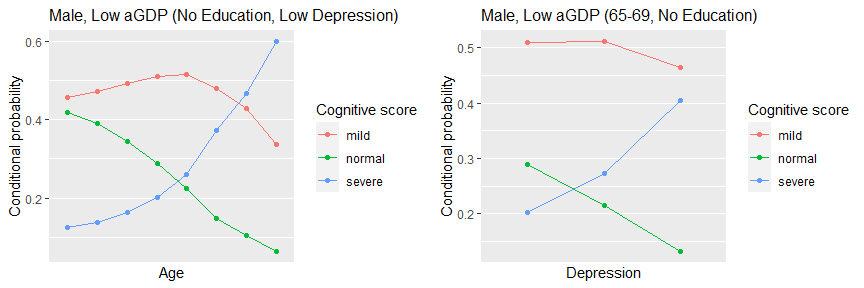
\includegraphics[width = \textwidth]{Images/summary.png}
	\caption{Examples of line graphs of cognitive impairment over age (left) and depression (right)}
	\label{summary}
\end{figure}

\clearpage

\begin{center}
\Large{Acknowledgments}
\end{center}

I am sincerely grateful to the supervisors of this project, Dr. Sara Wade and Dr. Cecilia Balocchi, as well as PhD supporter Steven Soutar, for their advice and guidance. I would also like to thank SHARE for providing the data and background information used in the research. 

This report uses data from SHARE Waves 1 \cite{share1}, 2 \cite{share2}, 3 \cite{share3}, 4 \cite{share4}, 5 \cite{share5}, 6 \cite{share6}, 7 \cite{share7}, and 8 \cite{share8}. The SHARE data collection has been funded by the European Commission, DG RTD through FP5 (QLK6-CT-2001-00360), FP6 (SHARE-I3: RII-CT-2006-062193, COMPARE: CIT5-CT-2005-028857, SHARELIFE: CIT4-CT-2006-028812), FP7 (SHARE-PREP: GA N°211909, SHARE-LEAP: GA N°227822, SHARE M4: GA N°261982, DASISH: GA N°283646) and Horizon 2020 (SHARE-DEV3: GA N°676536, SHARE-COHESION: GA N°870628, SERISS: GA N°654221, SSHOC: GA N°823782, SHARE-COVID19: GA N°101015924) and by DG Employment, Social Affairs \& Inclusion through VS 2015/0195, VS 2016/0135, VS 2018/0285, VS 2019/0332, and VS 2020/0313. Additional funding from the German Ministry of Education and Research, the Max Planck Society for the Advancement of Science, the U.S. National Institute on Aging (U01\_AG09740-13S2, P01\_AG005842, P01\_AG08291, P30\_AG12815, R21\_AG025169, Y1-AG-4553-01, IAG\_BSR06-11, OGHA\_04-064, HHSN271201300071C, RAG052527A) and from various national funding sources is gratefully acknowledged (see \href{www.share-project.org}{www.share-project.org}).

This report also uses data from the generated easySHARE data set \cite{easyshare}. The easySHARE release 8.0.0 is based on SHARE Waves 1, 2, 3, 4, 5, 6, 7 and 8.

\clearpage


\begin{center}
\Large{University of Edinburgh – Own Work Declaration}
\end{center}

This sheet must be filled in, signed and dated - your work will not be marked unless this is done.
\vspace{1cm}

Name: Yile Shi

Matriculation Number: s2168022

Title of work: Analysis on Dementia Risk Factors Based on Bayesian Networks

\vspace{1cm}

We confirm that all this work is my own except where indicated, and that We have:
\begin{itemize}
\item	Clearly referenced/listed all sources as appropriate	 				
\item	Referenced and put in inverted commas all quoted text (from books, web, etc)	
\item	Given the sources of all pictures, data etc. that are not my own				
\item	Not made any use of the report(s) or essay(s) of any other student(s) either past 	
or present	
\item	Not sought or used the help of any external professional academic agencies for the work
\item	Acknowledged in appropriate places any help that We have received from others	(e.g. fellow students, technicians, statisticians, external sources)
\item	Complied with any other plagiarism criteria specified in the Course handbook
\end{itemize}

We understand that any false claim for this work will be penalised in accordance with
the University regulations	(\url{https://teaching.maths.ed.ac.uk/main/msc-students/msc-programmes/statistics/data-science/assessment/academic-misconduct}).								

\vspace{1cm}

Signature:

\begin{figure}[!h]
	
\includegraphics[width = 0.5\textwidth]{Images/Signature.png}
\end{figure}

\vspace{5mm}

Date: 2022/6/30

\clearpage


% =============================================================================
% Table of contents, tables, and pictures (if applicable)
% =============================================================================
\pagestyle{plain}
\setcounter{page}{1}
\pagenumbering{Roman}

\tableofcontents

\pagenumbering{arabic}
\setcounter{page}{1}

\nocite{*}
\bibliographystyle{unsrt}
\clearpage

\section{Introduction}
\label{sec:intro}

Dementia, a clinical state characterized by loss of function in multiple cognitive domains, becomes a serious public health concern worldwide \cite{seixas2014bayesian}. Someone develops dementia every 3 seconds and current annual cost of dementia is estimated at 1 million dollars, which is set double in 2030 \cite{alzheimer2019world}. Because of the absence of effective treatment, prevention strategy to reduce dementia risk becomes an active research topic. This report aims to contribute to this topic by identifying potential risk factors behind dementia diagnosis. We expect that a better understanding of the influence of factors on cognitive impairment can help to inform the development of lifestyle interventions for dementia risk reduction. 

We apply exploratory data analysis on easySHARE dataset from Survey of Health, Ageing and Retirement in Europe (SHARE) and extract a sample of 57310 individuals recorded in 2013. Based on the subset, we build Bayesian networks and select the one with the best performance. Our goal is to find, among the following factors, the most likely to be relevant to cognitive decline: age; gender; country; education; drinking behaviour; smoking; obesity; physical activity; chronic disease; working status; household finance; social isolation; and depression. 

\section{Exploratory Data Analysis}  
\label{sec: EDA}

EasySHARE dataset is a combination of 8 waves of SHARE data recorded from 2004 to 2020, consisting of over 420k observations and 107 variables across various topics. It is inefficient to use all variables for modelling. On the other hand, from the summary of each column, we observe that the proportions of missing values in some columns are relatively high. For example, the variable \texttt{books\_age10} is only available in wave 3 and 5, hence a large amount of missing values is shown in figure \ref{fig:books_age10}.  Models using these features could loss much information on the data and result in inaccurate results. Thus, for model efficiency and accuracy, exploratory data analysis is necessary to explore the distribution of variables. We apply feature selection to drop redundant variables and feature transformation to define appropriate risk factors and response. Furthermore, as a result of cross-sectional research on a single wave, we extract a subset of data including these variables in a specific wave.

\begin{figure}[!h]
	\centering
	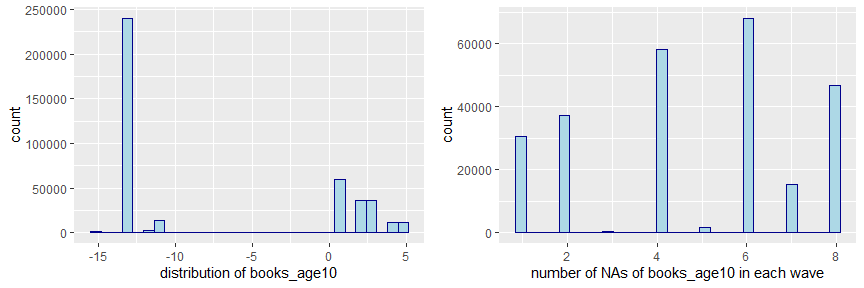
\includegraphics[width = 0.75 \textwidth]{Images/books_age10.png}
	\caption{Information of  \texttt{books\_age10}}
	\label{fig:books_age10}
\end{figure}

\subsection{Feature Selection}

\subsubsection{Risk Factors}

Referring to literatures of Crimmins et al (2011) \cite{crimmins2011assessment}, Beam et al (2018) \cite{beam2018differences} and Livingston et al (2020) \cite{livingston2017dementia}, we determine modifiable risk factors in 13 domains, including \textbf{age},  \textbf{gender}, \textbf{country}, \textbf{education}, \textbf{drinking behaviour}, \textbf{smoking}, \textbf{obesity}, \textbf{physical activity}, \textbf{depression}, \textbf{social connection}, \textbf{chronic disease}, \textbf{working status} and \textbf{household finance}. For each factor, we follow the variable descriptions in easySHARE data guide \cite{gruber2014generating} and select relevant variables following the rules below:

\begin{itemize}
	
	\item \textbf{Variables for the same risk factor should have less information overlapping}.
	
	Some risk factors have multiple relevant features. An appropriate combination of these variables can represent this factor properly. Nevertheless, combination using redundant variables with great overlaps possibly lead to model inefficiency and bias. For example, \texttt{euro1} to \texttt{euro12} are binary variables indicating if respondents had 12 specific mental feelings in the past respectively, while \texttt{eurod} is a composite scale of them. Thus, \texttt{eurod} is enough to represent the depression level.
	
	\item \textbf{Variables should contain missing values as few as possible.}
	
	Although constrain-based algorithms can deal with missing values automatically when constructing Bayesian networks, algorithm evaluation through cross-validation requires non-missing dataset. Using inconsistent datasets between algorithms will cause great bias. On the other hand, most imputation methods based on other columns are not suitable in this research, which probably increases the model errors when variables are not strongly correlated. Hot deck imputation using values from the same column in other waves also causes great bias as values in most variables probably change over the time. In this case, we have to drop incomplete observations from the dataset, so variables with fewer missing values are preferred as they keep the maximum information of the original data. 
	
	For example, considering one's social isolation,  \texttt{mar\_stat} and \texttt{partnerinhh} are both fine to represent this factor, while only one of them can be selected due to the former rule. Comparing the histograms \ref{fig:social}, we choose \texttt{partnerinhh} without missing values.
	
	\begin{figure}[!h]
		\centering
		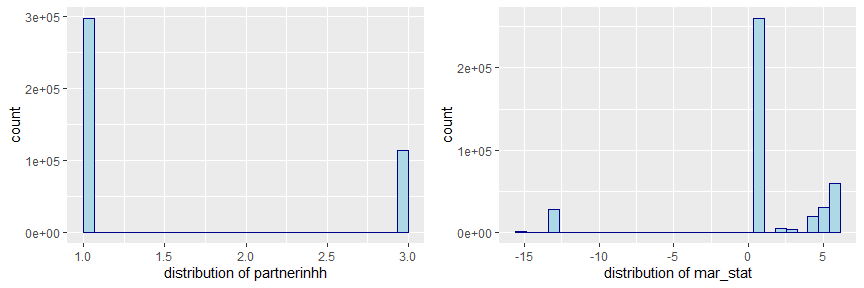
\includegraphics[width = 0.75 \textwidth]{Images/social.png}
		\caption{Distributions of \texttt{partnerinhh} and \texttt{mar\_stat}}
		\label{fig:social}
	\end{figure}
	
\end{itemize}

Table \ref{tab:vars} displays 13 variables selected to represent the risk factors based on the rules above.

\begin{table}[!h]
	\centering
	\begin{tabular}{|c|c|c|}
		\hline
		Risk Factor & Variables & Description \\
		\hline
		Age & \texttt{age} & age at interview \\ 
		Gender & \texttt{female} & gender of respondents \\
		Country & \texttt{country}  & country identifier\\
		Education & \texttt{isced1997\_r} & ISCED-97 coding of education status \\
		Drinking behaviour & \texttt{br010\_mod} & frequency of alcohol drinking \\
		Smoking & \texttt{smoking} & if respondents smoke at present \\
		Obesity & \texttt{bmi2} & categorized body mass index\\
		Physical activity & \texttt{br015\_} &  the frequency of vigorous activities \\
		Depression & \texttt{eurod} & scale of current depression \\
		Social connection & \texttt{partnerinhh} & if respondents live with spouse/partner \\
		Chronic disease & \texttt{chronic\_mod} & number of chronic diseases \\	
		Working status & \texttt{ep005\_} & current job situation \\
		Household finance & \texttt{co007\_} & confidence on household income \\
		\hline
	\end{tabular}
	\caption{Risk factors and corresponding variables}
	\label{tab:vars}
\end{table}

\subsubsection{Cognitive Score}

Next, we explore the variables corresponding to the model output. EasySAHRE dataset does not record diagnosis of dementia (e.g. Alzheimer's disease) in all waves. Instead, it contains the following indices to describe respondents' cognitive function:

\begin{itemize}
	\item \texttt{recall\_1}: the number of words recalled in the first trial of the word recall task, ranging from 0 to 10.
	\item \texttt{recall\_2}: the number of words recalled in the delayed word recall task, ranging from 0 to 10.
	\item \texttt{orienti}: orientation of date, month, year and day of week, ranging from 0 (good) to 4 (bad).
	\item \texttt{numeracy\_1}: information on the Mathematical performance, ranging from 1 (bad) to 5 (good).
	\item \texttt{numeracy\_2}: information on the second test on Mathematical performance, ranging from 0 to 5.
\end{itemize}

Following Crimmins' \cite{crimmins2011assessment}, we consider creating a composite cognitive score as the response variable in subsequent modelling, using these indices as a proxy for dementia severity. We visualize the distributions of these features in figure \ref{fig:cog_dist}:

\begin{figure}[!h]
	\centering
	\includegraphics[width = 0.8 \textwidth]{Images/cog_dist.png}
	\caption{Distributions of cognitive function indices}
	\label{fig:cog_dist}
\end{figure}

A high amount of missing values is observed in \texttt{orienti}, \texttt{numeracy\_1} and \texttt{numeracy\_2}. According to easySHARE guide, \texttt{orienti} and \texttt{numeracy\_1} have a large number of missing values in wave 4 to 8, while \texttt{numeracy\_2} is only available for respondents of wave 4 to 8 who already participated in one panel waves. Thus, for numeracy scores, only one of both is recorded in most observations. As mentioned, we do not apply imputation methods here and columns with fewer incomplete data are preferred. 

After variable selection, we consider extracting data of a specific wave from easySHARE dataset. Wave with more observations and higher proportion of complete data in each column is ideal. We compare data of aforementioned variables in 8 waves. For waves having over 20\% rows missing in \texttt{orienti}, we drop this column when comparing. For \texttt{numeracy\_1} and \texttt{numeracy\_2}, we pick either of them with more complete data and drop the other one. As a result, wave 5 is selected.

Furthermore, we drop the observations with \texttt{age} less than 50 as they are not the people of interest. We also notice that their exists a relatively small proportion ($<$0.2\%) of observations with values over 90 in \texttt{isced1997\_r} or \texttt{ep005\_}. According to easySHARE guide, these values represents the option \emph{others} and we also drop these observations. As a result, 57310 rows are kept for modelling.

\subsection{Feature Transformation}

Up to now, we have already extracted a subset including 17 variables in wave 5 from easySHARE dataset. Before subsequent modelling, we apply the following feature transformation steps on this subset:

\begin{enumerate}
	\item \textbf{Rename the variables for risk factors.}
		
	We rename most variables with the names of their corresponding risk factors to represent them, instead of abbreviations or numerical coding.
	
	\item \textbf{Create cognitive score as model response.}
	
	We create a composite cognitive score as the model response using corresponding indices. Since \texttt{orienti} and \texttt{numeracy\_1} has already been dropped, the cognitive score of a respondent is defined as the sum of \texttt{recall\_1}, \texttt{recall\_2} and \texttt{numeracy\_2}, ranging from 0 to 25. The higher the score is , the better cognitive function the respondent has. 
	
	\item \textbf{Discretize continuous nodes.}
	
	Due to the property of Bayesian Networks that discrete nodes only have discrete parents, we discretize continuous nodes so that they can be properly used. Referring to Livingston's (2020), the cognitive score is cut into 3 bins, based on its 10\% and 40\% quantiles, to represent severe impairment, mild impairment, and cognitively normal. Continuous nodes including age, chronic diseases and depression are discretized to ensure that each categories contains sufficient data in case of model overfitting. Figure \ref{fig:cog_age} shows the distributions of cognitive score and age, before and after discretization.
	
	\begin{figure}[!h]
		\centering
		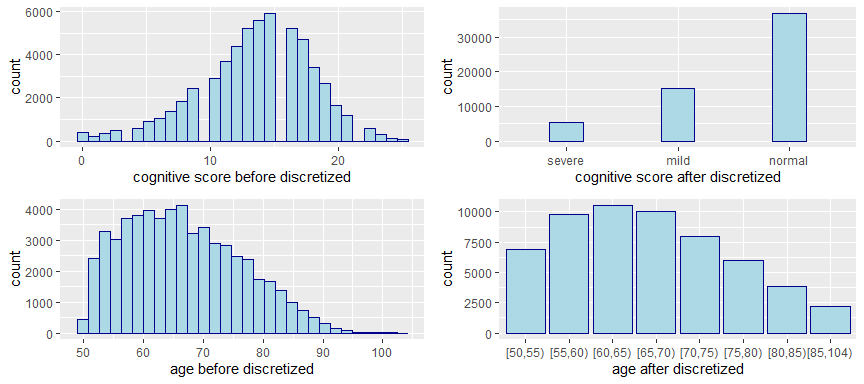
\includegraphics[width = 0.75 \textwidth]{Images/cog_age.png}
		\caption{Distributions of cognitive score and age}
		\label{fig:cog_age}
	\end{figure}
		
	Besides, country is also discretized to a binary variable. We refer to the average gross domestic product (aGDP) of relevant countries in 2013 when wave 5 was recorded and set a threshold of 40k dollars. Table \ref{tab:country_aGDP} shows countries with identifiers in each group. Figure \ref{fig:country} displays the distribution of country before and after discretization.
	
	\begin{table}[!ht]
		\centering
		\begin{tabular}{|c|c|}
			\hline
			1- High aGDP ($\geq$\$40k) & 0 - Low aGDP ($<$\$40k) \\
			\hline
			Austria (11) & Spain (15) \\
			Germany (12) & Italy (16) \\ 
			Sweden (13) & Israel (25) \\
			Netherlands (14) & Czech (28) \\
			France (17) & Slovenia (34) \\
			Denmark (18) & Estonia (35) \\
			Switzerland (20) & \\
			Belgium (23) & \\
			Luxembourg (31) & \\
			\hline
		\end{tabular}
		\caption{Countries categorized based on aGDP in 2013}
		\label{tab:country_aGDP}
	\end{table}

	\begin{figure}[!h]
		\centering
		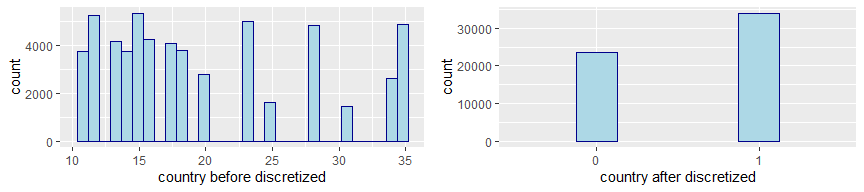
\includegraphics[width = 0.75 \textwidth]{Images/country.png}
		\caption{Distribution of country}
		\label{fig:country}
	\end{figure}
	
	\item \textbf{Recategorize some discrete factors.}
	
	Some categories of discrete factors, including education, drinking behaviour and physical activity, do not contain enough data, which leads to model overfitting. As a remedy, we recategorize these variables by combining some levels to ensure the number of observations in each stratification is sufficient. Figure \ref{fig:drinking} shows the distributions of drinking behaviour, before and after recategorized.
	
	\begin{figure}[!h]
		\centering
		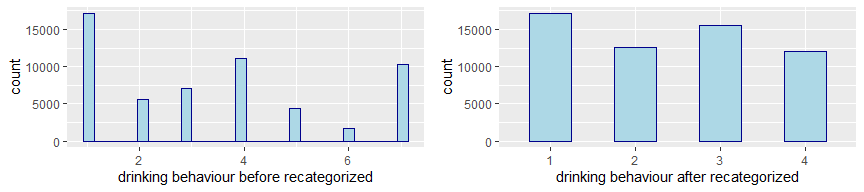
\includegraphics[width = 0.75 \textwidth]{Images/drinking.png}
		\caption{Distributions of drinking behaviour}
		\label{fig:drinking}
	\end{figure}
	
\end{enumerate}

After feature transformation, the subset is ready for subsequent modelling. Table \ref{tab:risk_score} shows the levels of risk factors and cognitive score.

\begin{table}[!h]
	\centering
	\begin{tabular}{|l|r|}
		\hline
		Risk factors & Levels \\
		\hline
		\multirow{2}{*}{Age} & 1: 50-54; 2: 55-59; 3: 60-64; 4: 65-69; \\
		 & 5: 70-74; 6: 75-79; 7: 80-84; 8: $\geq$85 \\
		 \hline
		Gender & 0: male; 1: female \\
		\hline
		Country & 0: low aGDP; 1: high aGDP \\
		\hline
		\multirow{3}{*}{Education} & 0: no education; 1: primary education; \\
		 & 2: lower secondary education; 3: secondary education; \\
		 & 4: post-secondary and tertiary education \\
		\hline
		Drinking behaviour & 1: never; 2: sometimes; 3: often; 4: almost everyday \\
		\hline
		Smoking & 0: no, 1: yes \\ 
		\hline
		Obesity & 1: underweight; 2: normal; 3: overweight; 4:obese \\
		\hline
		\multirow{2}{*}{Physical activity} & 1: more than once a week; \\
		 & 2: one to four times a month; 3: hardly ever, or never \\
		\hline
		Depression & 1: low; 2: medium; 3: high \\
		\hline
		Chronic diseases & 1: no disease; 2: one or two diseases; 3: over two diseases \\
		\hline
		\multirow{2}{*}{Working status} & 1: retired; 2: employed; 3: unemployed; \\
		 & 4: permanently sick or disabled; 5: homemaker \\
		\hline
		\multirow{2}{*}{Household finance} & 1: with great difficulty; 2: with some difficulty; \\
		 & 3: fairly easily; 4: easily \\
		 \hline
		Cognitive score & 1: severe; 2: mild; 3:normal \\
		\hline
	\end{tabular}
	\caption{Levels of risk factors and cognitive score}
	\label{tab:risk_score}
\end{table}

\clearpage

\section{Implementation}
\label{sec:implementation}

In this section, we introduce the Bayesian network and algorithms used for modelling. Moreover, we explain the evaluation of networks, and further the modification on the selected network.

\subsection{Bayesian Network}

The exposition in this subsection follows that in Scutari (2010) \cite{scutari2010learning}.

A Bayesian network is a probabilistic graphical model that represents a set of variables and their conditional dependencies via a directed acyclic graph (DAG). The graph is denoted by $\mathcal{G} = (V,E)$, where $V$ is the node set consisting of variables of interest and $E$ is the edge set. Each edge in $E$ represents a direct dependence between two noes.  For example, edge "A $\rightarrow$ B" means that node B depends on A. In this case, A is called the parent, while B is called the child. As name suggests, the graph supposed to be acyclic. Cycles such as "A $\rightarrow$ B $\rightarrow$ A" are not permitted. Table \ref{tab:bn_type} shows the 3 types of Bayesian networks:

\begin{table}[!h]
	\centering
	\begin{tabular}{|c|c|c|}
		\hline
		Type & Feature & Common choices of local distributions \\
		\hline
		Discrete & Only has discrete variables & Multinomial, Binomial, Poisson \\
		Continuous & Only has continuous variables & Multivariate normal, Student-t, Beta \\
		Mixed & Has both discrete and continuous variables & - \\
		\hline
	\end{tabular}
	\caption{Types of Bayesian networks}
	\label{tab:bn_type} 
\end{table}

Bayesian network analysis starts with structure learning, which has two categories of algorithms:
\begin{itemize}

\item \textbf{Constraint-based algorithms}: these algorithms learn the network structure by analysing the probabilistic relations entailed by the Markov property of Bayesian networks with conditional independence tests (e.g. mutual information) and then constructing a graphs satisfying the corresponding d-separation statements. The common choices could be \emph{Peter-Clark (PC)} algorithm, and \emph{Incremental Association (IAMB)} algorithm.

\item \textbf{Score-based algorithms}: these algorithms assign a score (e.g. Bayesian Information Criteria) to each candidate Bayesian network and try to maximize it with some heuristic search algorithm. \emph{Hill-climbing (HC)}, based on greedy search algorithms, is the common choice.

\end{itemize}

Next, a blacklist and a whitelist are defined, based on general information and expert knowledge, to avoid or ensure some edges in the network. We define the blacklist following the rules below:

\begin{itemize}
	\item No arrow starts from the response node, cognitive score.
	\item No arrow points to nodes of respondents' natures, i.e. age, gender or country.
	\item As an early-life factor, education is only possibly influenced by age, gender and country.
\end{itemize}

We define the whitelist with two edges "working status $\rightarrow$ household finance" and "social isolation $\rightarrow$ depression" based on our common sense.

\subsection{Evaluation of Algorithms}

We now evaluate the performance of structure learning algorithms including \emph{PC}, \emph{IAMB} and \emph{HC}. For each algorithm, we calculate the average loss for the response node, cognitive score, through 10-fold cross-validations on the extracted subset. Classification error is implemented as the loss function, because most loss functions, including mean squared error, are not available in discrete networks.Values of cognitive score are predicted using the information present in its local distribution from its parent nodes. Lower value of the loss indicates better performance. Considering the random effect of cross-validation, we repeat computing average loss of each algorithm with different random seeds. As shown in table \ref{tab:bn_cv}, network based on HC over-performs the other two algorithms. Therefore, HC is selected for further modification and estimation. Figure \ref{fig:hc} displays the initial Bayesian Network based on HC.

\begin{table}[!h]
	\centering
	\begin{tabular}{|c|c|c|c|c|c|}
		\hline
		algorithm & seed = 1 & seed = 2 & seed = 3 & seed = 4 & seed = 5 \\
		\hline
		PC & 0.3285017 & 0.3273365 & 0.3285484 & 0.3274023 &  0.3276248 \\
		IAMB & 0.3231999 & 0.3242536 & 0.3238454 & 0.3234789 & 0.3229207 \\
		HC & 0.3226488 & 0.3224045 & 0.3230326 & 0.3227360 & 0.3227883 \\
		\hline
	\end{tabular}
	\caption{Average loss of algorithms after 10-fold cross-validation with different random seeds}
	\label{tab:bn_cv}
\end{table}

\begin{figure}[!h]
	\centering
	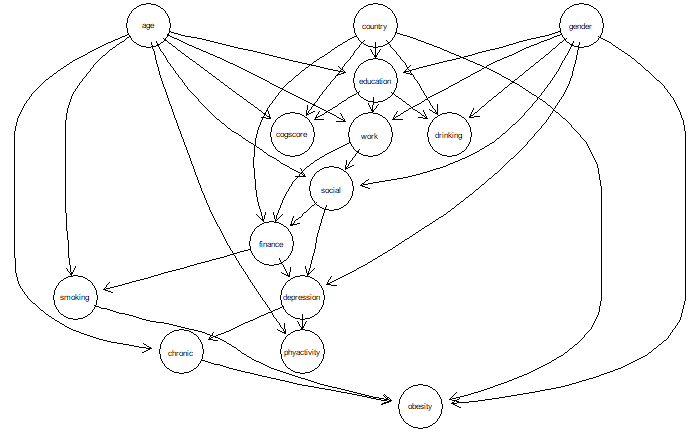
\includegraphics[width = 0.65 \textwidth]{Images/hc.png}
	\caption{Initial Bayesian network created using HC algorithm}
	\label{fig:hc}
\end{figure}

\subsection{Model Modification}

 The network above may miss some edges of interest as algorithms do not exhaust all possible edges. Besides, casual effects indicated in some edges violates our general knowledge, although they are statistically significant. Thus, the network need further modification to make it more reasonable. Unlike constraint-based algorithms, HC doesn't require conditional independence test before any modification. We compare model performance after all modifications are finished.

First, we drop the edge "household finance $\rightarrow$ smoking" as we do not believe the financial status of the household affects one's smoking habit directly. Similarly, edges "education $\rightarrow$ drinking behaviour" and "depression $\rightarrow$ physical activity" are dropped. Besides, we reverse the edge "depression $\rightarrow$ chronic disease" following the logic that physical diseases influence individual's mental health.

Next, we add the edge "gender $\rightarrow$ cognitive score" into the network as gender is believed to have significant effect on respondents' cognition according to \cite{beam2018differences}. Moreover, since all risk factors are assumed to have direct or indirect effect on individual's cognitive function through at least one path, we add the edges "depression $\rightarrow$ cognitive score", "obesity $\rightarrow$ depression", "physical activity $\rightarrow$ obesity" and "drinking behaviour $\rightarrow$ obesity" to ensure the assumption holds. 

We calculate the average loss of modified networks through 10-fold cross-validations, and compare the results with the initial network. We repeat the computation with different random seeds to reduce the random effect of cross-validations. The results are shown in table \ref{tab:hc}:

\begin{table}[!h]
	\centering
	\begin{tabular}{|c|c|c|}
		\hline
		seed & before & after \\
		\hline
		1 & 0.3226488 & 0.3191122 \\
		2 & 0.3224045 & 0.3198102 \\
		3 & 0.3230326 & 0.3190773 \\
		4 & 0.3227360 & 0.3192692 \\
		5 & 0.3227883 & 0.3184842 \\
		\hline
	\end{tabular}
	\caption{Average classification error of the network before and after modification}
	\label{tab:hc}
\end{table}

As a result, the modified network performs better and is selected for subsequent estimation and interpretation.

\clearpage

\section{Results}
\label{sec:results}

The modified Bayesian network based on Hill-climbing algorithm is determined as the final network, shown in figure \ref{fig:hc_mod}.  As the parents of cognitive score, \textbf{age}, \textbf{gender}, \textbf{country}, \textbf{education} and \textbf{depression} tend to have significant effects on respondents' cognitive function. 

\begin{figure}[!h]
	\centering
	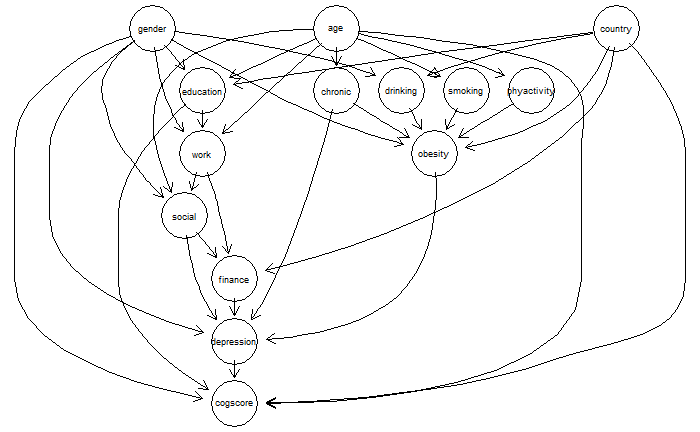
\includegraphics[width = 0.75 \textwidth]{Images/hc_mod.png}
	\caption{Final Bayesian network}
	\label{fig:hc_mod}
\end{figure}

Next, we estimate the parameters of local distributions of these parent nodes. We use the classical Bayesian posterior estimator with imaginary sample size of 10000, which provides smoother and more robust estimates, comparing with the alternative method using maximum likelihood estimation. We plot line graphs to explore the trends of the conditional probabilities of cognitive score, conditioning on its parent nodes. Since model overfitting happens in stratifications with sparse counts when conditioning on too many nodes, plots of the basic model are wiggly. As a remedy, we apply ordered logistic regressions of cognitive score, grouped by gender, over other parent nodes. Figure \ref{fig:smoothing} displays the improvement of line graphs after using ordered logistic regression.

\begin{figure}[!h]
	\centering
	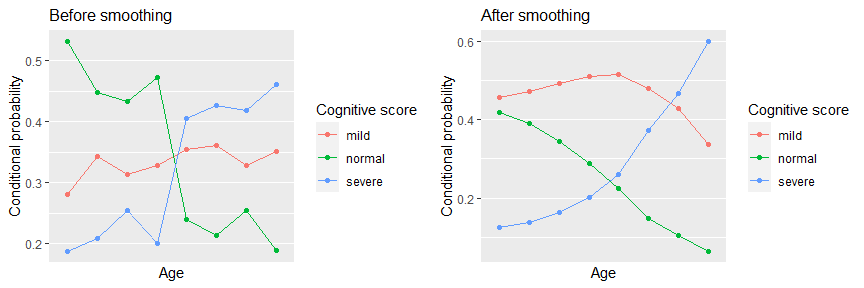
\includegraphics[width = \textwidth]{Images/smoothing.png}
	\caption{Line graphs for same data before and after smoothing}
	\label{fig:smoothing}
\end{figure}

With smoother line graphs, we discuss the influence of parent nodes on dementia risk:

\subsection{Age}

Age shows a negative influence on individual's cognitive function from the line graphs. Generally, as respondents age, the conditional probability of having severe cognitive impairment increases, while the probability of being cognitively normal drops. This is consistent with our common sense. As people get older, they suffer from worse health condition and more loneliness, which could lead to cognitive decline. The path "age $\rightarrow$ chronic diseases $\rightarrow$ depression $\rightarrow$ cognitive score" in the network supports this view. 

We condition on people's education and depression level. Given a specific gender group, we observe better cognitive function among respondents from countries with high aGDP in all age groups, as they have higher probability to be cognitively normal and lower probability to have severe cognitive impairment than those from countries with low aGDP. On the other hand, looking at individuals from the same country group, female respondents show higher chance to suffer from severe cognitive impairment than males, especially in higher age groups (e.g. over 85). Figure \ref{fig:age1} displays the trends of cognitive score over age in different gender and country groups, among respondents with no education and low depression level.

\begin{figure}[!h]
	\centering
	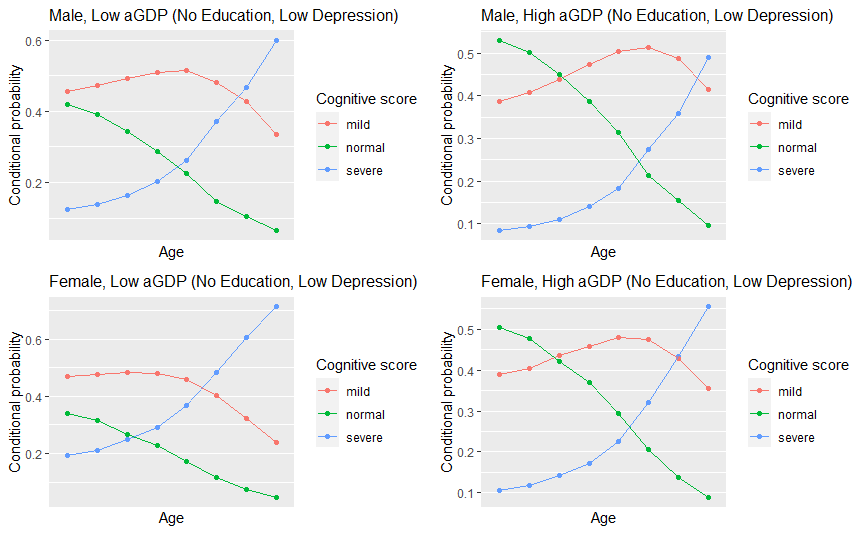
\includegraphics[width = \textwidth]{Images/age1.png}
	\caption{Trends of cognitive score over age (no education and low depression level)}
	\label{fig:age1}
\end{figure}

Interestingly, we notice that most lines become steeper after 65 yeas old, indicating faster decline on people's cognition. Thus, we think that 65 could be an important time point where individual's cognitive decline aggregates. This is consistent with results from the study of Lee et al (2018) \cite{lee2018association} in China. Furthermore, we particularly focus on the influence of other factors in the age groups around 65.

\subsection {Education}

Education level tends to have a positive effect on dementia risk reduction. According to line graphs, conditional probability of severe cognitive impairment decreases when respondents have higher education levels, and these people have higher chance to be cognitively normal. It has been proved that education, as a main contributor, stimulates people's cognitive function in early life according to the work of Black et al (2018) \cite{blacker2018brain}. Besides, individual's education level might influence the work and further the income in midlife, which are also believed to have effects on cognition in other researches \cite{livingston2017dementia}.

Similarly, we condition on age and depression level here. In each gender group, though the trends of lines are very similar, people from countries with low aGDP seems to have higher dementia risk, due to lower conditional probability of being cognitively normal and higher probability of having severe impairment on cognition. In each country group, again, female respondents could be more likely to suffer from cognitive impairment, particularly in low education levels. Figure \ref{fig:edu1} shows the trends of cognitive score over education levels in different gender and country groups, holding 65-69 yeas old and low depression level.

\begin{figure}[!h]
	\centering
	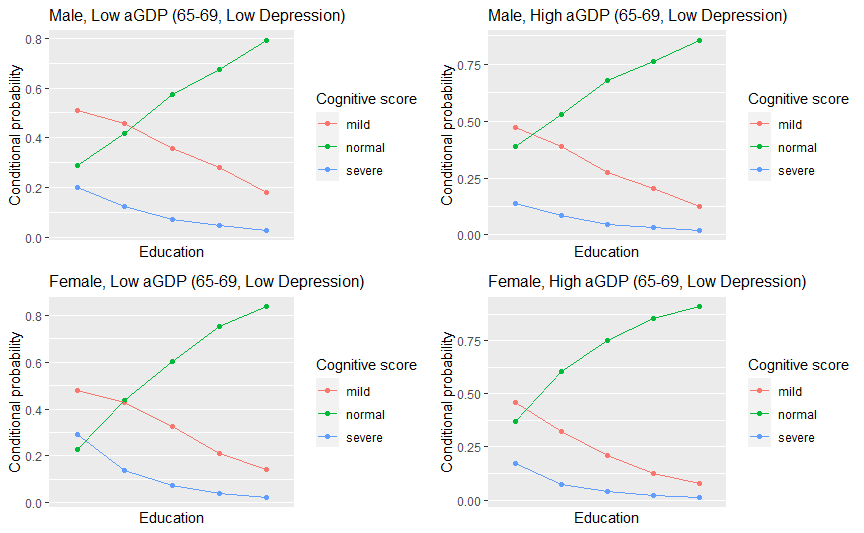
\includegraphics[width = \textwidth]{Images/edu1.png}
	\caption{Trends of cognitive score over education (65-69 years old, low depression level)}
	\label{fig:edu1}
\end{figure}

\subsection{Depression}

Depression is found to aggravate individual's cognitive impairment. From the line graphs, we observe that as depression level increases, the conditional probability of normal cognition drops and people are more likely to suffer from severe cognitive impairment. As a part of the prodrome and early stages of dementia, depression is associated with various possible psychological or physiological mechanisms. This can be supported by edges corresponding to depression across many domains in the network including "social $\rightarrow$ depression", "household finance $\rightarrow$ depression, "chronic diseases $\rightarrow$ depression" and "obesity $\rightarrow$ depression".  Poor health condition, low income and social isolation all tends to cause the feeling of depression, and further influence individual's cognition.

Given age, gender and education level, the conditional probability of normal cognition of respondents from countries with high aGDP is significantly higher than those from countries with low aGDP at each depression level. Accordingly, the probability of suffering from severe cognitive impairment in countries with high aGDP is much lower than it in the other stratification. Conditioning on the country group, we find that women possibly have higher dementia risk than men from the plots. Figure \ref{fig:depression1} shows the trends of the conditional probabilities of different cognitive function levels over depression, holding 65-69 age group and no education level.

\begin{figure}[!h]
	\centering
	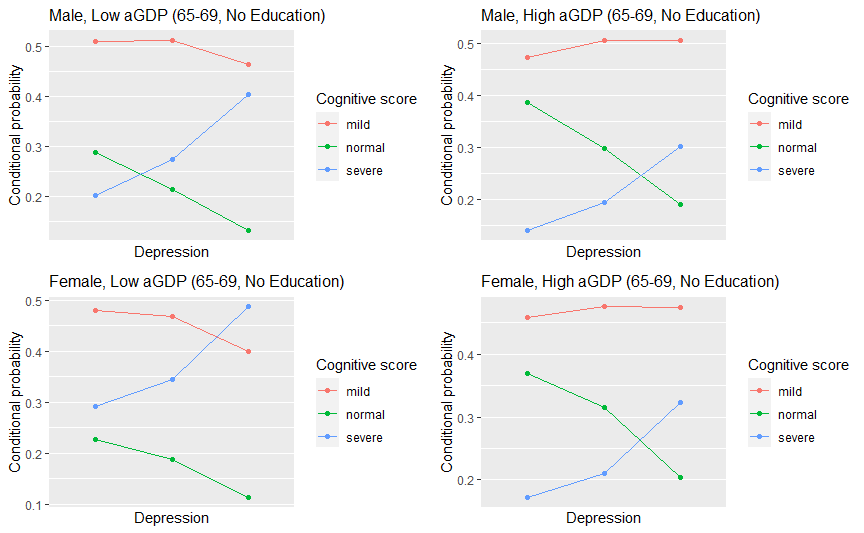
\includegraphics[width = \textwidth]{Images/depression1.png}
	\caption{Trends of cognitive score over depression (65-68 years old, no education)}
	\label{fig:depression1}
\end{figure}

Moreover, we notice that segments from medium to high depression level become much steeper than those from low to medium level. According to the ranges of depression levels, respondents with at least 5 negative feelings are determined with high depression. Thus, we guess it could be a threshold that people experiencing over 4 negative feelings have much higher dementia risk than others.

\subsection{Gender}

Gender shows consistent influence on cognitive function across analysis on age, education and depression that generally females have higher dementia risk than males, holding other factors constant. In particular, this difference is observed to be more significant in elder age groups. These results are consistent with the conclusions in \cite{beam2018differences}.  A possible explanation for females having higher probabilities of cognitive impairment may be that women generally survive to longer ages than men, making the proportion of women become larger in elder groups. On the other hand, due to their longevity, female respondents are more likely to live alone. This could result in more severe social isolation, increases their depression level and finally affects their cognition, which is supported by the path "female $\rightarrow$ social isolation $\rightarrow$ depression". Besides, we believe that gender could affect individual's cognitive function in other ways including the education level and obesity, from the network.

\subsection{Country}

Recall that we divide countries into two groups, based on their average gross domestic product in 2013. According to previous analysis, we conclude that respondents from countries with high aGDP tend to have lower dementia risk than those from countries with low aGDP. The influence of country can be various. From the network, we observe that country are significantly associated with nodes including education, obesity, drinking behaviour and household finance. Generally, countries with high aGDP probably have better welfare, which means they could provide higher-standard education and more advanced health care for their citizens than other countries, positively affecting the cognitive function. Moreover, provided with better welfare, people in these countries may live with more joy, hence they have lower depression level, which also reduces the probability of cognitive decline.

\clearpage

\section{Conclusions}

We construct a modified Bayesian network on a subset of easySHARE dataset to identify risk factors on dementia. As a result, age, gender, country, education and depression tend to have significant influence on individual's cognitive function. Specifically, the probability of severe cognitive impairment rises as age or depression level increases. In particular, individuals over 65 years old or experiencing high-level depression have much higher dementia risk. Education shows opposite influence on cognitive function that people with higher education levels have lower risk. Gender and country affect individual's cognition in a variety of ways. Generally, females have higher dementia risk than males; people from countries with low aGDP have higher probability to suffer from dementia.

There are some limitations of this research. First, although hearing loss, diabetes, and hypertension are believed to have important effect on cognitive impairment in \cite{livingston2017dementia}, their influence could not be identified due to the lack of relevant columns in easySHARE data. We could only define a general factor "chronic diseases" to count the number of chronic diseases the respondents had and explore its possible influence on dementia risk instead. To determine the specific effects of these diseases, we need to access data with relevant variables. Second, our research belongs to cross-sectional analysis, which focuses on data at a specific time point among different individuals and obtains conclusions for the general population. In this case, our research is lack of the exploration on longitudinal effects of some risk factors on dementia risk among particular respondents over the time.

\clearpage

%the entries have to be in the file literature.bib
\bibliographystyle{unsrt}
\bibliography{literature}
\clearpage

\appendix
\section*{Appendix}
\addcontentsline{toc}{section}{Appendix}

Programming part in this research is completed with R. 

\subsection*{R packages:}

For EDA section, we use the \texttt{tidyverse} and \texttt{gridExtra} packages. We construct and estimate the networks with \texttt{bnlearn} package and display the network with \texttt{Rgraphviz} package. \texttt{MASS} package is used to fit the ordered logistic regression on cognitive score. All histograms and line graphs are generated with \texttt{ggplot2}.

\subsection*{R code: }
The complete code is available via this \href{https://github.com/Shi-Yile/Project-1-Dementia-Risk-Factors.git}{Github repository}.

\clearpage

\section*{Word Count}
\addcontentsline{toc}{section}{Word Count}

This report contains 4828 words, including executive summary, main text, references and appendix. The screenshot using  \texttt{Analyse Text} function in TeXstudio is provided.

\begin{figure}[!h]
	\centering
	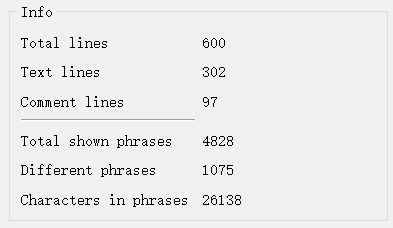
\includegraphics{Images/word_count.png}
	\caption{Word count in TeXstudio}
\end{figure}

\end{document}
